%!TEX root = ../dissertation.tex

\begin{savequote}[75mm]
Potential energy is just a word. It only has meaning if we provide it. For example, does this pen have potential energy?\newline
::picks up pen and then drops it onto the floor::
\qauthor{Dr. Philipp Preiss}
\end{savequote}


\chapter{Optical Lattices and \newline the Bose-Hubbard model}
\label{sec:ch1}

%\footnotetext{\footnotemark \footnotemark I love my colleague's quote here. Partially because it represents a feeling every AMO graduate student feels at some point, but also because of how close our bonds with atom's should be -- perhaps quite literally.}

Ultracold neutral atoms in optical lattices provide a new paradigm in the ability to experimentally simulate quantum models. The level of control that can be applied to neutral atoms enables physicists to realize these quantum systems in their absolute ground states and create nearly defect free lattice potentials engineered out of laser light. Additionally, the physical length scale of this physics admits the possibility of microscopic resolution of all degrees of freedom within a given measurement basis. 

Such a framework for a quantum mechanical model maps most directly to condensed matter systems where the atom in the optical lattice takes the place of an electron in a crystal \cite{Jaksch1998}. For the sake of brevity, we will skip over most of the experimental footwork necessary to get to the point where such a relationship can be made. Instead, I will simply state that such a mapping is possible as long as the atoms can be made ultracold ($\sim 1\mathrm{nK}$) \cite{Bakr2010,Bakr2011,Preiss2015}. The average energy, or temperature, of the atom needs to be comparable to the kinetic energy and interaction energies within the optical lattice to probe the same physics. Another way of seeing the same relationship is to see if the thermal deBroglie wavelength, $\lambda_{th}$, of the atom is on the order of the lattice constant $a$ such that it may be in a coherent superposition of occupying many lattice sites simultaneously and indistinguishable from other atoms within neighboring lattice sites. In our system, the quoted temperature provides $\lambda_{th} \approx 6 \mathrm{\mu m} $ which is $\approx 10$ lattice sites. With this crude justification in mind, we will now derive the physics of a particle being described as a wave in such a periodic potential.

\section{Single-particle physics in optical lattices}

Optical coupling of orbital electronic states in neutral atoms provide a mechanism for both conservative and dissipative forces \cite{Metcalf1999}. These two processes can be thought of as elastic and inelastic scattering, respectively, of photons with the atom. The dissipative force is provided by the absorption of a photon or emission of a photon and has been famously used for trapping and cooling of atomic gases\cite{Chu1986,Raab1987,Chu1998,Metcalf1999}. However, the vast majority of all work and models discussed in this thesis will rely on tailoring conservative potentials with almost arbitrary spatial control\cite{Ashkin1970,Metcalf1999,Grimm2000}. Since the only external forces that interact with the atoms are optical and predominantly conservative, the system remains, to a very good approximation, isolated from the surrounding external environment.

\subsection{Neutral atoms in optical potentials}

A neutral atom experiences a conservative external potential from optical photons when the frequency of the light is far from the atomic resonance. This light, rather than being absorbed by the atom, induces an electric dipole moment in the atom. The amplitude of the alignment, or anti-alignment, of this dipole moment with the external electrical field changes the energy of the atom and is known as the ac-Stark shift\cite{Ashkin1970}. In the case of a two-level atom in a monochromatic laser field, where the laser detuning is large enough that the rotating wave approximation can be used, the conservative potential provided by the dipole atom-light interaction is given by: 

\begin{equation}
\label{eqn:Vdipole}
	V_{dipole} (r) \approx \frac{3\pi c^2}{2 \omega_o^3}\frac{\Gamma}{\Delta} I(r)
\end{equation}


where the atomic transition frequency is $\omega_o$, the linewidth of the transition is $\Gamma$, the intensity of the laser power is $I(r)$, and the detuning of the laser frequency from the atomic transition is $\Delta = \omega-\omega_o$. Note that the both the laser intensity, $I(r)$, and the detuning, $\Delta$, are complimentary ways to change dipole potential depth. Additionally, the sign of the detuning $\Delta$ controls whether the atom is attracted to or repelled from the high-intensity locations of the laser beam profile. This is commonly referred to as either red- or blue-detuning of the laser with respect to the atomic transition frequency due to their association with the colors in the visible spectrum. While (\ref{eqn:Vdipole}) is written for a two-level atom approximation, additional energy levels can be included to provide a more accurate response \cite{Metcalf1999}.

However, even an off-resonant laser illuminating the atom does not act purely as a conservative potential since the photons still have a finite probability to exchange energy and momentum with the atom\cite{Grimm2000}. The likelihood of such a dissipative process depends on both the intensity of the light, $I$, and the laser detuning with respect to the linewidth of the atomic transition $\Gamma/\Delta$. The rate at which an atom scatters light is given by (\ref{eqn:gscatter}):

\begin{equation}
\label{eqn:gscatter}
	\Gamma_{sc}(r) \approx \frac{3 \pi c^2}{2 \hbar \omega_o^3} \left ( \frac{\Gamma}{\Delta} \right )^2 I(r) = \frac{1}{\hbar} \frac{\Gamma}{\Delta} V_{dipole}(r)
\end{equation}

By detuning the laser far from resonance, we see that the scattering rate, or dissipative contribution of the light-atom interaction, is reduced compared to the conservative contribution by a factor of $(\Gamma/\Delta)$. This implies that for the same desired dipole potential depth $V_o$, it is always favorable to increase both the laser detuning and the intensity to reduce the scattering rate to more faithfully realize a purely conservative potential. This consideration of these two scalings provide some guidance in how to choose practical parameters for the lasers that produce the desired optical potentials (see \S \ref{sec:ch2_heating}). 

%In the case of $~^{87}$Rb, the two relevant optical transitions come from the D1 and D2 lines of the $5s\rightarrow6p$ transition which occur at $\lambda=795$nm and $\lambda=780$nm respectively. All attractive, red-detuned, potentials in this work are derived from a broadband $\lambda\approx840$nm SLED source\footnote{EXALOS bladdy blue}. All repulsive, blue-detuned, potentials are derived from a similar broadband $\lambda\approx758$nm SLED source\footnote{EXALOS bladdy blue2}. We will predominantly study Hamiltonians provided purely by this repulsive light.

\subsection{Bandstructure and Bloch wave functions}

All experiments in this thesis will be realized in an effective $1$-D optical lattice that is generated from interfering blue-detuned light. The potential generated from this light depends on the intensity of its interference pattern and is written as:

% If, in terms of energy seen by the atom, each beam provides $(V_o/2) e^{\pm i k x - i \omega t}$, then the potential given is by: 

\begin{equation}
\label{eqn:Vpot}
V(x)=-(V_o/2) \cos{\left ( 2 k_l x \right )}
\end{equation}

where $k_l$ \footnote{This k-vector ($k_l$) is defined as $2\pi/\lambda$ when the light used to create the potential originates from two counter-propagating lasers where $\lambda$ is the laser wavelength. However, this only provides an upper-bound for what k-vector can be produced by a given laser wavelength. What matters is the k-vector in the plane of the lattice formed by the lasers which can be tuned by their relative angle. This point will be further elucidated in \S \ref{sec:qgm}.} is the wavevector (or k-vector) of the laser light used to create the potential. The potential has been written with zero DC average for mathematical convenience. The total Hamiltonian then for a single-particle is written as:
%\begin{equation}
%\label{eqn:lattlight}
% $\left ( (V_o/2) e^{i k x-i \omega t} + (V_o /2) e^{-i k x - i \omega t})^2 = V_o/2 (e^{i 2 k x} + 2 + e^{- i 2 k x} \right )$
%\end{equation}

\begin{equation}
\label{eqn:HamBS}
H=\frac{\hat{p}^2}{2m}+V(x)
\end{equation}

where $m$ is the mass of the atom. In the case of zero lattice depth, $V_o=0$, this Hamiltonian realizes a single-particle in free space whose eigenstates are described by a propagating wave with an eigenenergy that depends only on its momentum $\hbar k$: $\psi_k = e^{i k x/\hbar}$. A side note is that this potential-free Hamiltonian has a continuous translational symmetry in space and therefore conserves momentum which additionally implies that eigenstates of this Hamiltonian are also eigenstates of the momentum operator, $\hat{p}$. \footnote{This is, of course, obvious since the Hamiltonian is composed of only the momentum operator $\hat{p}$. However, the statement about symmetries and invariance relating to conserved quantities is a general one.\cite{Weinberg2015}}

Once the lattice depth is non-zero, this symmetry is broken such that the Hamiltonian only retains a discrete translational symmetry. The Bloch theorem states that since the Hamiltonian (\ref{eqn:HamBS}) has a discrete translational symmetry from the periodic potential (\ref{eqn:Vpot}), then the eigenfunctions of the Hamiltonian will also be eigenfunctions of this discrete translation and hence will also be periodic (\ref{eqn:blochFx}).

\begin{equation}
\label{eqn:blochFx}
\phi_q^{(n)} (x) = e^{i q x/\hbar} \cdot u_q^{(n)}(x)
\end{equation}

The Bloch wave functions, $\phi_q^{(n)}$, are labeled by their band index $n$ (which will become apparent later) and their quasi-momentum, or crystal momentum, $q$. This quasi-momentum is akin to the linear momentum of the free-particle case referenced to above except that it is now only defined within the Brillouin zone of the periodic potential $- \hbar k_l \leq q \leq \hbar k_{l}$ where $k_l$ is the k-vector of the laser light. The function $u_q^{(n)}(x)$ is a Fourier series with a periodicity that correspond to integer multiples of the lattice period. Intuitively, the high-frequency cut off for $q=\pm \hbar k_l$ for defining $\phi^{(n)}_q(x)$ derives from the periodic potential that can only ``detect" or ``sample" spatial variation with a frequency equal to or less than its own.\footnote{This is akin to Nyquist frequency if you are an electrical engineer.} Note that this does not define that the Bloch wave function cannot have local spatial variation with higher frequencies than the lattice periodicity, just that whatever this local high-frequency variation is, it must repeat periodically with the lattice period. The remaining slowly varying envelope function is then defined by $e^{iqx/\hbar}$.\footnote{The presence of these high-frequency variations come through the Fourier series of $u_q^{(n)}(x)$ and will be apparent in the higher bands defined by the index $n$, which are related to the free-particle momentum states centered about an integer $n$ of $k_l$ displacements of momentum in Fourier space.}

To find the eigenfunctions of this new Hamiltonian with momentum states coupled by integer multiples of the lattice k-vector ($k_L=2 k_l$), we can more conveniently solve this problem in Fourier space and solve for the eigenergies $E_q^{(n)}$. We first write both the potential and the periodic function $u_q^{(n)}(x)$ as Fourier series:

\begin{equation}
\label{eqn:FSV}
V(x) = \sum_m V_m e^{i 2 m k_l x/\hbar}
\end{equation}

and

\begin{equation}
\label{eqn:ux}
u_q^{(n)}(x) = \sum_r c_r^{(n,q)} e^{i 2 r k_l x/\hbar}
\end{equation}

The periodic potential term $V(x)$ in (\ref{eqn:FSV}) only has two non-zero terms that correspond to the lattice periodicity $ \left ( V_{m=-1} = V_{m=1} = -V_o / 4 \right ) $. To find the coefficients for the Fourier series of $u_q^{(n)}$ and the eigenenergies $E_q^{(n)}$, one should exploit the orthogonality relation between Fourier modes after taking the inner-product of $\langle e^{i 2 r' k_l x/\hbar} | H | \phi_q^{(n)} \rangle$. This procedure results in:

\begin{equation}
\label{eqn:HamC}
\sum_{r'} H_{r,r'} \cdot c_r^{(n,q)} = E_q^{(n)} c_r^{(n,q)}
\end{equation}

where

\begin{equation}
\label{eqn:HamLL}
H_{r,r'} = \left \{
\begin{array}{ll}
   (2 r + q / k)^2 ,& r=r' \\
   -V_o/4, & | r-r' | = 1 \\
   0, & otherwise \\
\end{array} 
\right .
\end{equation}

Diagonalizing the Hamiltonian (\ref{eqn:HamLL}), where $r$ and $r'$ are matrix indices, will solve for the eigenenergies that depend on the continuous variable $q$ and the discrete index $n$ which labels the characteristic formation of \emph{bands} in the spectrum. To gain some intuition for the system this Hamiltonian describes, we can again first think about the $V_o=0$ case. In the case of no external potential, this Hamiltonian will realize a parabolic dispersion curve in $k$-space from the momentum of a free-particle. By turning on the lattice potential, $V_o \neq 0 $, the external potential can now provide momentum ``kicks" to the particle's wave function in discrete quanta of $2\hbar k_l$ (when the indices $r,r'$ differ by $1$). In the case that the energy from the free-particle dispersion curve at $q$ and $q\pm 2\hbar k_l$ are $\lesssim V_o$, then these two momentum states are strongly coupled and these states hybridize to form an eigenstate composed of a superposition of the two free-particle states. The first time this happens is at the $q=\pm \hbar k$ point in the dispersion curve and defines what is known as the Brillouin zone boundary in a crystal. Physically, this hybridization corresponds to perfect Bragg reflection of the particle's wave function at the Brillouin zone boundary. This hybridization forms the familiar \emph{gaps} associated between bands of energy as defined on a reduced Brillouin zone band diagram (\ref{fig:freePartBS}). Note that this also introduces a natural energy scale for this physics known as the lattice recoil energy. In essence, the Braggs scattering is an elastic scattering event by two photons within the plane of the lattice that change the momentum of the particle in the lattice. For a given light k-vector defined in the plane of the lattice, $k_l$, this gives us the recoil energy defined as:

\begin{equation}
E_r = \frac{~~(\hbar k_l)^2}{2 m}
\label{eqn:Er}
\end{equation}

\begin{figure}[t!]
		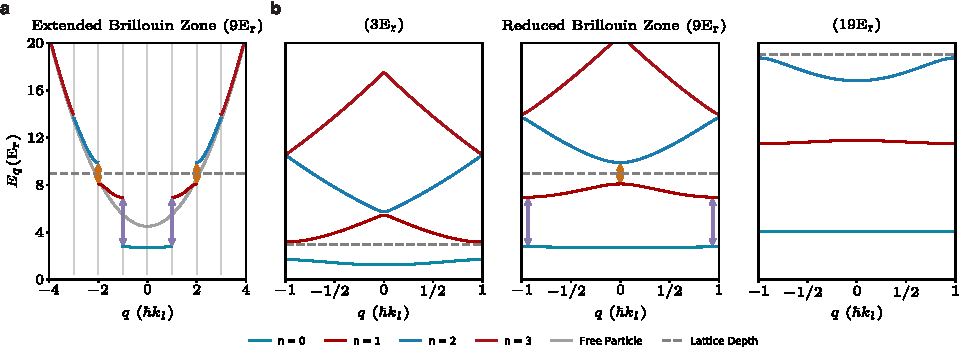
\includegraphics[width=\columnwidth]{figures/ch1/BandStructure/BZ_BS_v2_edit.pdf} 
		\caption{\textbf{Dispersion with Bragg reflection. a)} The left curve shows free-particle dispersion parabola (gray line) and the formation of gaps in the Bloch wave functions from Bragg scattering off the lattice. Additionally, the dashed-grey lines show the height of the lattice as it is centered about zero and determines when a state $| \psi_k^{(n)} \rangle$ is bound to the lattice. This depiction of the hybridization of the free-particle dispersion curve is known as the extended Brillouin zone scheme and is an intuitive way of how to reach the notion of bands from Bragg scattering. \textbf{b)} The reduced Brillouin zone scheme is associated with condensed matter physics and band structure and more common in the literature. This mapping is both compact and conceptually reflects the notion of periodic states that are described by Bloch wave functions $| \phi_q^{(n)} \rangle$ that are only well defined for quasi-momentum states $q$ that are bounded by the lattice wave-vector $k_L$.}
		\label{fig:freePartBS}	
\end{figure}

Once the lattice depth, $V_o$, is deep enough that an entire band lies within its energy window, it conceptually makes sense to describe these as Bloch functions that are bound to the lattice. These original free-particle states are now sufficiently dressed by Bragg reflected states with momenta that differ by integer multiples of the lattice vector $\hbar k_L=2\hbar k_l$ that they form a stationary wave with particle density maxima that reside deep in the potential minima. This is shown for both the ground band and the first excited band in in Fig.~\ref{fig:freePartBS}. This thesis will use the convention that $n=0$ refers to the ground band. These periodic eigenstates of the Hamiltonian are plotted for various quasi-momentum states for both the ground band and the excited band in Fig.~\ref{fig:blochFX}. A common physical picture given for the opening of a gap at the edge of the Brillouin zone, in the weak lattice limit, is given by the phase of the Bloch wave function's spatial structure. While,

\[
 \left | \phi_{q=\hbar k}^{n=0,1} (x) \right \rangle \approx e^{i k_l x/\hbar} + (-1)^n e^{-i k_l x/\hbar}
 \]
 
 are both composed of the same free-particle momenta states, their symmetric versus anti-symmetric superposition either concentrates the density of the particle either in the minima or the maxima of the lattice potential (as shown in Fig.~\ref{fig:blochFX}). This provides an obvious energy difference between the two combinations purely by the overlap of the wave function and the lattice potential -- the kinetic energies should be approximately the same.

\begin{figure}[t!]
		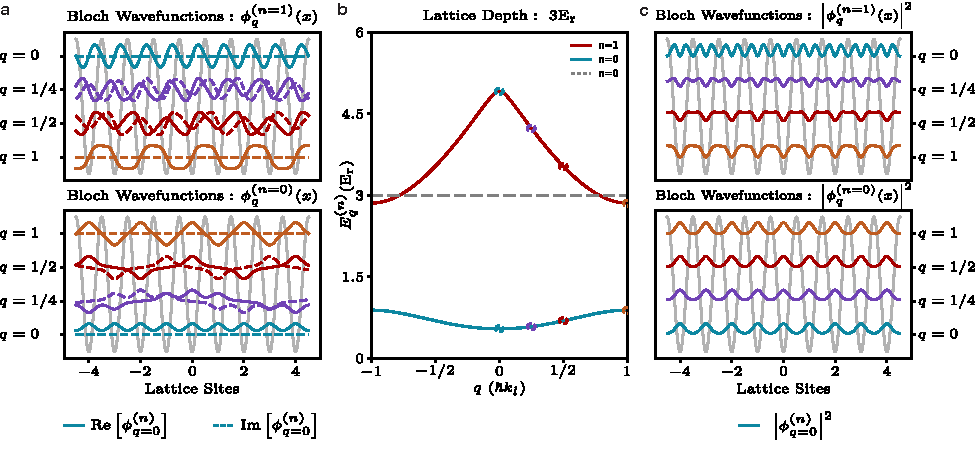
\includegraphics[width=\columnwidth]{figures/ch1/blochFx/BlochFunctionsBS2_v2edit.pdf} 
		\caption{\textbf{Bloch wave functions. a)} The left plots depict the real and imaginary parts of the Bloch wave function's ($ | \phi_q^{(n)} (x) \rangle$) spatial dependence as a function of distance for various quasi-momenta and both the $n=0$ and $n=1$ bands at a lattice depth of $4E_r$. \textbf{b)} Plots the band structure for at $4E_r$ and the quasi-momenta the plotted Bloch wave functions describe. \textbf{c)} These right plots depict the density distribution of the Bloch functions for the same quasi-momenta as the left plots and same bands. Note that only the ground-band, $n=0$, is entirely bound to the lattice and relatively ``flat". Unlike the $n=0$ band, $n=1$ band has a significant deviation in its wave function across the band and has lots of particle probability that does not lie in the minima of the potential well and reflects its unbound nature.}
		\label{fig:blochFX}	
\end{figure}

There are two primary quantities that are typically extracted from the band structure due to their physical relevance: the band width and the band gap. The band width, the energy difference between the maximum and minimum energy for a given band $\left ( \argmax_q {\left \{ E_q^{(n)} \right \}}- \argmin_q { \left \{ E_q^{(n)} \right \} } \right)$, describes the maximum kinetic energy of a particle confined to that band. The kinetic energy becomes substantially suppressed as bands become bound to the lattice and will appear to be approximately flat. The band gap, the energy difference between successive bands $\Delta = E_q^{(n+1)} - E_{q'}^{(n)} $, defines how well separated a particle in one band is energetically from another band. Practically speaking, all the physics in this thesis will assume a single-band model where all particles inhabit the ground-band of the lattice. This makes the band gap a relevant metric for determining how well the observed phenomena will be described by a single-band Hamiltonian and how susceptible the system will be to some form of heating that deposits energy into the system. The evolution of the band gap and band width can be seen from progression of band structure plots in Fig.~\ref{fig:bandGaps} as well as the evolution of the band gaps between various successive bands as a function of lattice depth.

\begin{figure}[t!]
		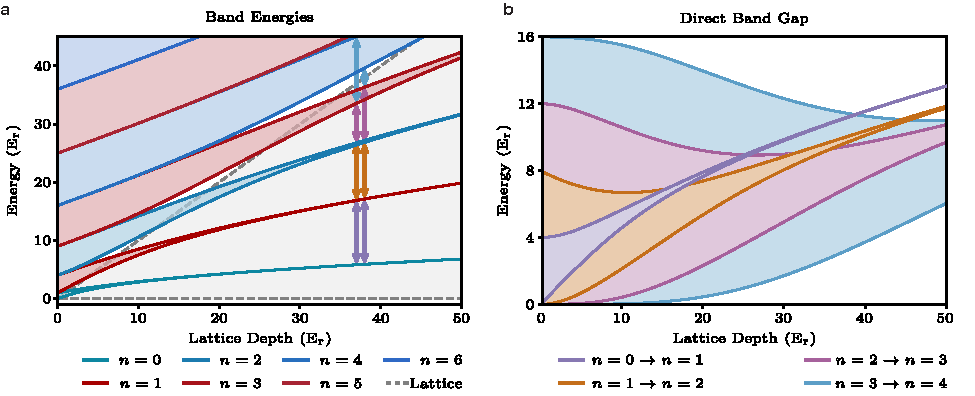
\includegraphics[width=\columnwidth]{figures/ch1/BandStructure/BSScaleV2_edit.pdf} 
		\caption{\textbf{Band Gaps. a)} The band structure of the four lowest bands are plotted for three lattice depths to depict how both the band widths and band gaps change as a function of lattice depth. Note that the lower bands both flatten and become gapped from the excited bands more quickly as a function of lattice depth. \textbf{b)} The band gap between successive bands can strongly depend on which quasi-momentum is being excited from and to $\left ( \Delta_{q,q'}^{n,n+1}=E_q^{(n)}\rightarrow_{q'}^{(n+1)} \right )$. In principle both direct, quasi-momentum preserving, and indirect, non-quasi-momentum preserving, excitations are possible in a lattice. However, in the case of a simple sinusoidal lattice, both the minimum and maximum band gaps are captured by just analyzing direct band excitations. The minimum and maximum band gaps are plotted as the solid lines and the distribution of all intermediate possible values are plotted as the shading.}
		\label{fig:bandGaps}	
\end{figure}

\subsection{Wannier wave functions}

The Bloch wave functions, as the single-particle eigenstates, are a natural and convenient way to describe the physics of a particle in a periodic potential. They are a complete set of energy eigenstates and completely described by their band index $n$ and quasi-momentum $q$. Since they are defined by a single quasi-momentum number $q$, they are maximally localized in momentum space and maximally delocalized in position space. A useful alternative, orthonormal basis for this system is given by the set of functions that describe the particle as localized in position space. These set of functions are known as Wannier functions and are a convenient way to describe the wave function of a particle in a band $n$ that is maximally localized at a lattice site $x_i$. This basis can be constructed from a superposition of all Bloch wave functions within the Brillouin zone for a given band $n$:

\begin{equation}
w_n(x-x_i) = \frac{1}{\mathcal{N}} \sum_q e^{-i q x_i} \phi_q^{(n)} (x)
\label{eqn:wnfx}
\end{equation}.

The normalization factor $\mathcal{N}$ depends on the finite number of quasi-momentum Bloch wave functions summed over. Additionally, since the Bloch wave functions are eigenstates of the original Hamiltonian, they may have been solved with an arbitrary global phase that will become an important relative phase in the construction of the Wannier functions $w_n(x-x_i)$. Thankfully, there is a convenient recipe to follow that establishes how to choose the phases when constructing $w_n(x-x_i)$ that produces a wave function maximally localized on site $x_i$.

We have seen from the symmetry of the periodic potential, the hybridization of the free-particle states at the edge of the Brillouin zone, and the plots of the Bloch functions in Fig.~\ref{fig:blochFX} that the wave functions of even bands ($ n = 2\times m, m\in \mathbb{Z}$) are also even functions of $x$ and the wave functions of odd bands are also odd functions of $x$. The Wannier functions will also retain this symmetry since they are constructed from the Bloch functions within a given band. To then construct a maximally localized wave function at lattice site $x_i$, we must find the necessary phases multiplied by the Bloch wave functions that constructively add at $x=x_i$. For even bands, we choose a phase for each Bloch function that makes it both real and positive at $x=x_i$. \footnote{It does not actually matter which phase you pick for this site, just that you rotate all Bloch wave functions such that their phase is the same at $x=x_i$ : $Arg \left [ \phi_q^{(n)} \right ] = const.$ $\forall$ $q$, where $const. \in \mathbb{C}$} For odd bands, the Bloch wave functions are also odd about the center of each lattice site $x=x_i$. The recipe used above is modified such that the phase chosen is such that the first derivative of the Bloch wave functions are real and positive at site $x_i$. Including the recipes described above we can write down the Wannier functions construction as follows:

%$(Arg \left [ \phi_q^{(n)}(x) |_{x=x_i} \right ] = const.)$.
%$(Arg \left [ \partial \phi_q^{(n)}(x)/dx |_{x=x_i} \right ] = const)$

\begin{equation}
\label{eqn:wFx}
w_n(x-x_i) = \left \{
\begin{array}{ll}
   \frac{1}{\mathcal{N}} \sum_q e^{\left ( - i Arg [ \phi_q^{(n)} (x_i) ] \right )} \cdot \phi_q^{(n)} (x), & n\mathrm{\text{ is even}}\\
   \frac{1}{\mathcal{N}} \sum_q e^{\left ( - i Arg [ \partial \phi_q^{(n)} (x)/ \partial x |_{x=x_i} ] \right )} \cdot \phi_q^{(n)} (x), & n \mathrm{\text{ is odd}}\\
\end{array} 
\right .
\end{equation}

The Wannier wave functions represent the maximally localized, conjugate basis to the Bloch wave functions. These Wannier states become more localized for increasing lattice depth, which is plotted in Fig.~\ref{fig:wFx}\textbf{a} for the ground band. We can additionally see in Fig.~\ref{fig:wFx} that for a $45 \mathrm{E_r}$ lattice how the Wannier wave functions are also successively wider for higher bands in the lattice. 

\begin{figure}[t!]
		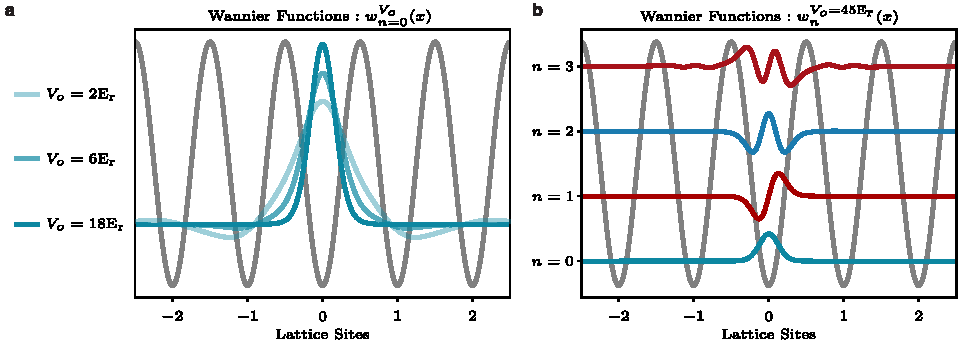
\includegraphics[width=\columnwidth]{figures/ch1/BHParams/WannierFx_v2edit.pdf} 
		\caption{\textbf{Wannier wave functions. a)} The Wannier wave functions for the ground band ($n=0$) are plotted for three different optical lattice depths. Note that this is plotted in the \emph{field} of the Wannier function, not the density distribution of the atom on a given site. \textbf{b)} The Wannier wave functions are plotted here for band indices $n=[0,3]$ for a deep lattice depth of $V_o=45 \mathrm{E_r}$. Note that they are closely approximated by the harmonic oscillator solutions in this regime.}
		\label{fig:wFx}	
\end{figure}

%A few useful observations can also be made from both the analytical form of $w_n(x-x_i)$ (\ref{eqn:wFx}), the bands from which they are constructed (Fig.~\ref{fig:freePartBS}) that coincide with their plots in Fig.~\ref{fig:wFx}. Since successively higher bands are mapped from a higher, but limited range, of free particle momenta, we see that $w_n(x-x_i)$ must contain only Fourier components that correspond to the range $n \cdot \hbar k_L \leq k \leq (n+1) \cdot \hbar k_L$. Hence, the Wannier functions for successively higher bands, while still maximally localized, contain a corresponding wrapping of the wave function by $n \cot \pi$. 

A useful, limiting case observation is that as the lattice depth becomes much larger than the band width of a given band, the Wannier functions approach the wave functions of a Harmonic oscillator, as can be seen by the similarity between the $w_n(x-x_i)$ plotted in Fig.~\ref{fig:wFx}b and Hermite Gaussians solutions of the Harmonic oscillator.\footnote{This is additionally a conceptually comforting fact as the cosine potential providing the lattice can be approximated to lowest order as a quadratic potential. However, due to the finite depth of the lattice, there is always a non-negligible amplitude in the wings of $w_n(x-x_i)$ that is necessary for an accurate description of the system.} This also implies that the Wannier functions become increasingly approximated by a superposition of free-particle states with a Gaussian envelope centered at an integer number of Bragg scattering events defined by the band index $n \times 2 \hbar k_l$. Lastly, while the Wannier functions are not eigenstates of the original Hamiltonian, they become asymptotically close as $V_o \rightarrow \infty$, where both the corresponding band becomes flatter and the associated Bloch wave functions will be nearly degenerate.

\section{The Bose-Hubbard model}

The treatment for deriving band structure and Bloch wave functions describes the entire physical story for a single-atom in an optical lattice. However, it neglects the many-body physics associated with interacting particles that leads to celebrated exotic condensed matter systems. It additionally does not easily lend itself to describing the nature of inter-particle interactions that are often derived from a local, inter-particle potential. To incorporate these local dependencies, we will now reformulate the free-particle Hamiltonian from before into a local basis that utilizes our derivation of the Wannier functions in the previous section.

In particular, we will describe the overlap of an atomic wave function with a local Wannier function defined about a particular lattice site as the population of the atoms in an orbital defined about that site. This leads us towards adopting the tight-binding lattice model for bosonic particles that is known as the Bose-Hubbard model. This is a renowned toy condensed matter model that faithfully incorporates strong inter-atomic interactions that lead to strongly correlated states that are otherwise absent in interaction corrected mean-field equations, such as the Gross-Pitaevski equation \cite{Preiss2015, Jaksch1998}. 

\subsection{Interacting atoms in an optical lattice}

In all our experiments, we work with dilute atomic gases. In these dilute gas regimes, the atom-atom interactions can be described be an effective inter-atomic potential between any two particles $V(\textbf{r})$, where $\textbf{r}$ is the inter-particle distance. This potential is strongly repulsive at distances on the order of a few Bohr radii, $(\sim a_o)$, due to the strong Coulomb interaction between the respective atom electron clouds. However, since atoms are polarizable, they are attractive at long distances due to the mutually induced dipoles that lead to a van der Walls force \cite{Weiner1999}. 

In the case of the low temperatures utilized by ultracold atom experiments, these inter-atomic interactions primarily result in elastic scattering processes between the atoms. In this regime, it is not necessary to know the exact shape of the interatomic potential since the low kinetic energies of the atoms do not enable them to probe past the centrifugal barrier. This means that only the lowest partial wave scattering process, \emph{s}-wave scattering, significantly contributes to the inter-atomic interactions. Therefore, this contribution can be well approximated by a contact interaction that is characterized by a single parameter that quantifies the \emph{s}-wave scattering length, $a_s$: 

\begin{equation}
\label{eqn:UCPot}
V(\textbf{r})=\frac{4 \pi \hbar^2 a_s}{m} \delta (\textbf{r})
\end{equation}

These interactions are often tunable via Feshbach resonances where the interaction strength can be changed by many orders of magnitude and even change sign \cite{Chin2010}. Additionally, it can be tuned through a much narrower range via the lattice depth by increasing the wave function overlap between atoms.

\subsection{Deriving the Bose-Hubbard model parameters}
\label{sec:ch1HO}

We can derive the Bose-Hubbard model by incorporating the inter-atomic contact interactions into the Hamiltonian of a bosonic field $\hat{\Psi}(\vec{x})$ \footnote{Note that by using this many-bodied bosonic field operator $\hat{\Psi}(\vec{x})$, we have implicitly moved into a second-quantized notation. This means that later when we populate this bosonic field with individual atoms as quantized excitations in the field ($\hat{a}^\dagger$), we have assumed these excitations to be indistinguishable from one another and will correctly incorporate the symmetrization necessary to accommodate these quantum statistics.} and an external potential:

\begin{equation}
\begin{aligned}
H =  & \int d^3 x~\hat{\Psi}^\dagger (\vec{x}) \left ( -\frac{\hbar^2}{2m} \nabla^2 + V(\vec{x}) \right ) \hat{\Psi}(\vec{x}) ~\\
& + \frac{1}{2} \frac{4 \pi \hbar^2 a_s}{m} \int d^3 x \int d^3 x' ~\hat{\Psi}^\dagger (\vec{x}) \hat{\Psi}^\dagger (\vec{x}') \delta(\vec{x}-\vec{x}') \hat{\Psi} (\vec{x}) \hat{\Psi} (\vec{x}')
\end{aligned}
\label{eqn:BHHL}
\end{equation} 

where $\vec{x}=\left ( x_1, x_2, x_3 \right )$.

Here the potential contains both the lattice potential and any additional potential term applied on top of the lattice that is relatively weak and spatially varies more slowly than the lattice itself: $V(\vec{x})=V_{latt}(\vec{x}) + V_{arb}(\vec{x})$. In the low temperature regime, the atoms only populate the ground band and we can restrict this derivation to involving only basis states that overlap with this band. Since the interaction term is entirely local it is convenient to expand the bosonic field $\hat{\Psi}(\vec{x})$ in terms of ground band Wannier wave functions:

\begin{equation}
\label{eqn:wfh}
\hat{\Psi}(\vec{x}) = \frac{1}{\mathcal{N}} \sum_i \hat{a}_i w_o(\vec{x}-\vec{x}_i)
\end{equation}

Here $\hat{a}_i$ $(\hat{a}^\dagger_i)$ are the annihilation (creation) operators for a boson in the ground band Wannier function centered at a lattice site $\vec{x}_i$. These operators follow the typical bosonic commutation relation $ [\hat{a}_i, \hat{a}_j^\dagger]=\delta_{i,j}$. This expansion allows us to rewrite (\ref{eqn:BHHL}) in terms of these bosonic annihilation and creation operators:

\begin{equation}
\begin{aligned}
H = - \sum_{i,j} J_{i,j} \hat{a}_i^\dagger \hat{a}_j + \sum_{i,j,k,l} \frac{U_{i,j,k,l}}{2} \hat{a}_i^\dagger \hat{a}_j^\dagger \hat{a}_k \hat{a}_l + \sum_i (h_i - \mu) \hat{a}^\dagger_i \hat{a}_i
\end{aligned}
\label{eqn:BHM}
\end{equation}

The additional potential that was added on top of the lattice, $V_{arb}(\vec{x})$, provides a variation in the on-site energy potential $h_i$. The chemical potential $\mu$ is a thermodynamic quantity that constrains the total particle number in the grand canonical ensemble description of the model. The $J_{i,j}$ term is known as the tunneling matrix element quantifies the tunneling rate between any two sites $i$ and $j$ and describes the kinetic energy of the atom. The $U_{i,j,k,l}$ term describes the various interaction matrix elements between atoms on sites $i,j,k,l$. Although the Wannier functions are constructed as an orthonormal basis, they were never eigenstates of the original Hamiltonian. Formally then, we can quantify these matrix elements via the overlap of the Wannier functions after the Hamiltonian has acted on them: 

\begin{equation}
J_{i,j} = - \int d^3 x ~ w^*_0 (\vec{x}-\vec{x}_i) \left ( - \frac{\hbar^2}{2m} \nabla^2 + V_{latt}(\vec{x}) \right ) w_0(\vec{x}-\vec{x}_j) 
\label{eqn:J}
\end{equation}

\begin{equation}
U_{i,j,k,l} = \frac{4 \pi \hbar^2 a_s}{m} \int d^3 x ~ w^*_0 (\vec{x}-\vec{x}_i) w^*_0 (\vec{x}-\vec{x}_j) w_0(\vec{x}-\vec{x}_k) w_0(\vec{x}-\vec{x}_l)
\label{eqn:U}
\end{equation}

\begin{figure}[t!]
		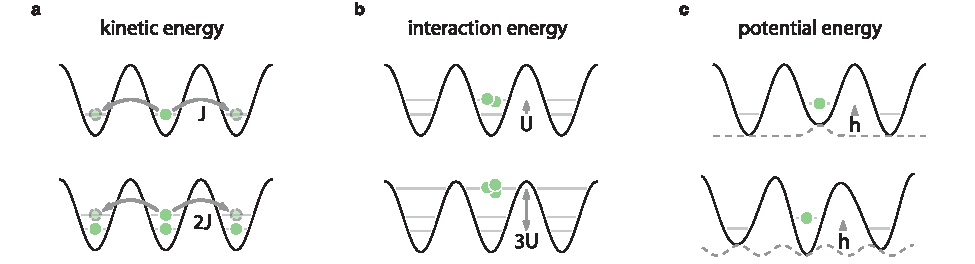
\includegraphics[width=\columnwidth]{figures/ch1/bh_cartoons/bh_cartoon.pdf} 
		\caption{\textbf{Bose-Hubbard terms. a)} Each green disk represents a bosonic atom excitation of the many-body wave function that populates a Wannier function centered on a given lattice site $x_i$. The kinetic energy term $J$ describes the coupling, or hopping rate, of the Wannier wave function to neighboring sites. In the presence of multiply occupied sites, this is energetically increased by bosonic enhancement. \textbf{b)} The interaction energy for multiply occupied sites is non-linear in the on-site occupation number $\hat{n}_i$ since it depends upon the number of pair-wise scatterings on a given lattice site. \textbf{c)} On-site lattice potential variation, either intentional or unintentional, adds an additional energetic parameter for locally tuning the Bose-Hubbard model with optical potentials due to disorder or confining trap potentials.}
		\label{fig:BHCartoon}	
\end{figure}

For nearly all practical cases, we will work in the ``tight-binding" regime of this ground band model. This approximation assumes that the Wannier functions are sufficiently localized that all higher order tunneling processes and higher order interaction terms may be ignored. This leaves the model with only a nearest-neighbor tunneling $J_{i,i\pm1}\equiv J$ and on-site interaction $U_{0,0,0,0}\equiv U$ and results in the standard form of the celebrated Bose-Hubbard model:

\begin{equation}
H_{BH} = - J \sum_{\langle i,j \rangle} \hat{a}^\dagger_i \hat{a}_j + \frac{U}{2} \sum_i \hat{n}_i (\hat{n}_i-1) + \sum_i (h_i - \mu) \hat{n}_i
\label{eqn:BHC}
\end{equation}

where $\hat{n}_i = \hat{a}_i^\dagger \hat{a}$ is the on-site number operator and the bracket sum, $\langle i,j \rangle$, refers to a sum only over neighboring indices. Physically, the mechanism that describes the exact contributions for the on-site interaction term comes from the sum of all pair-wise interactions of $n$ atoms on site $i$, each of which contribute an energy cost of $U$ : $U \sum_i {\hat{n}_i \choose 2} = U \sum_i \frac{\hat{n}_i!}{(\hat{n}_i-2)! 2!} = \frac{U}{2} \sum_i \hat{n}_i \left ( \hat{n}_i-1\right )$. All of these processes are illustrated below in Fig.~\ref{fig:BHCartoon}.

Both parameters J and U change significantly as a function of the lattice depth $V_o$. The qualitative features of the states that are harbored by the Bose-Hubbard model depend only on the ratio of these two quantities $U/J$. Practically speaking, the absolute energy scales of these two parameters are important for defining relevant experimental time-scales. This conversion comes from defining all energies by $\hbar$ as an \emph{angular} frequency. In our experiment, the depth of the lattice is measured in lattice recoil $E_r/\hbar \approx 2\pi \times 1240 \mathrm{Hz}$ and sets these overall energy scales. The values for J and U, as calculated from the ground state Wannier wave functions (\ref{eqn:J}, \ref{eqn:U}), are plotted for the parameters of our experimental parameters in Fig.~\ref{fig:BHP}. 

\begin{figure}[t!]
		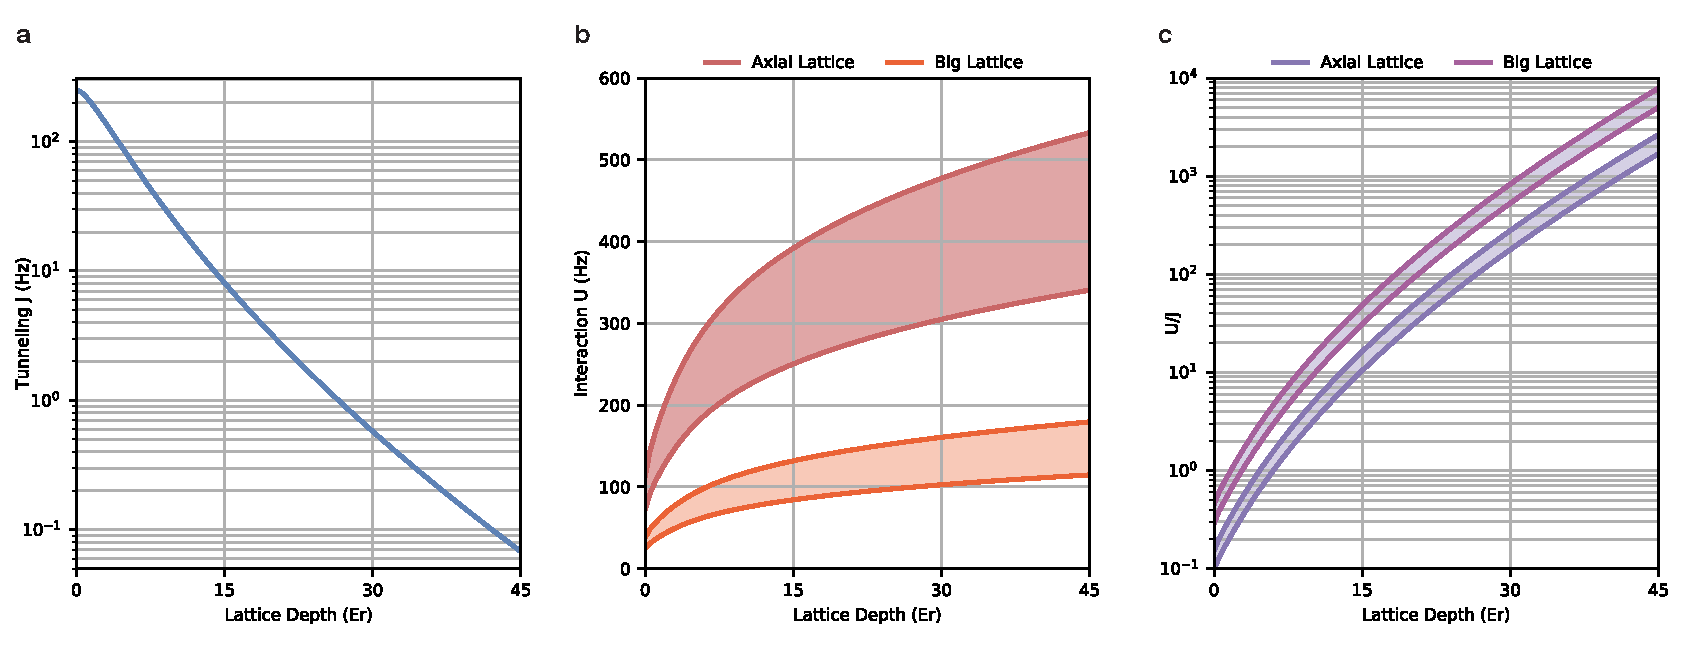
\includegraphics[width=\columnwidth]{figures/ch1/BHParams/BHParams_2.pdf} 
		\caption{\textbf{Bose-Hubbard Parameters. a)} The hopping parameter $J$ is evaluated for the optical lattice used in our experiments and is plotted here as a function of lattice depth. \textbf{b)} The interaction energy $U$ is plotted as a function of lattice depth for a one-dimensional system. The absolute energy scale requires the knowledge of the amount of confinement in the other two spatial dimensions. The band of possible values plotted here relies on the two different $z$-confining optical lattices that each have different spacings and can be varied through different amounts of optical powers. This translates into a variable amount of compression of the wave function and hence interaction strength U. \textbf{c)} This plot shows the relevant ratio of $U/J$ which qualitatively determines the physics investigated in the system. This plot is also for a one-dimensional system. }
		\label{fig:BHP}	
\end{figure}

In the deep lattice (tight-binding) limit, the dispersion of the ground band becomes well approximated by a cosine potential: $E_q = - 2 J \cos{\left (2 \pi q/k_l \right )}$ where $J$ is the Bose-Hubbard hopping parameter. In this regime, the analytical form for $J$ can be solved for exactly and approximately decays exponentially with lattice depth:

\begin{equation}
\label{eqn:tightJ}
J = \frac{4}{\sqrt{\pi}} E_r \left ( \frac{V_o}{E_r} \right )^{3/4} e^{-2 (V_o/E_r)^{1/2}}
\end{equation}

 Additionally, the scaling of $U$ with lattice depth can be estimated by approximating Wannier wave functions with the Harmonic Oscillator Gaussian states. In this limit the two relevant comparisons to the lattice can be given by the effective on-site trap frequency $\omega_{ho}$ and oscillator length $l_{ho}$ that depend on the lattice depth:
 
\begin{equation}
\label{eqn:w_ho}
\omega_{ho} = 2 E_r \sqrt{V_o/ E_r}
\end{equation}

\begin{equation}
\label{eqn:l_ho}
l_{ho}=\sqrt{\hbar / m \omega_{ho}} = \frac{a/2}{2\pi} \left ( \frac{V_o}{E_r} \right )^{-1/4}
\end{equation}

\begin{equation}
\label{eqn:wnHO}
w_n(x-x_i) \approx \psi_{l_{ho}}^n = \frac{1}{\sqrt{2^n n!}} \left ( \frac{1}{\pi l_{ho}^2} \right )^{1/4} e^{-x^2/(2 l_{ho}^2)} H_n (x / l_{ho})
\end{equation}

where $H_n(x/l_{ho})$ are the Hermite polynomials of order $n$.

This leads to an approximate scaling of $U\propto V_o^{1/4}$. This elucidates the point that while both $J$ and $U$ are tunable with lattice depth, the relevant ratio of $U/J$ is mostly determined by the exponential suppression of $J$ with the lattice depth. However, one crucial difference is that $J_{x,y,z}$ should be defined per lattice direction and depends only on the lattice depth along this direction. This is not the case for $U$ which depends upon the integral of the Wannier wave function in all three dimensions. This means that even without using a Feshbach resonance, there is some marginal tunability of $U$ by just changing the lattice depth in the dimensions orthogonal to the dimension of interest for $J$. This is particularly relevant since the majority of the work described in this thesis is performed for one dimension. The lattices that provide confinement along the $z$-direction has the widest range of tunability and is plotted in Fig.~\ref{fig:BHP} as two-bands of experimentally accessible ranges for one-dimensional Bose-Hubbard physics parameters.

%Intuitively it then makes sense that the time evolution operator from this Hamiltonian acting on any Wannier function will now inherently break this orthogonality.

%we are using second quantization

\section{Quantum phase transitions: superfluid to Mott-insulator}

Quantum phase transitions are a celebrated achievement in physics that differ from their classical counterparts since they can occur even at zero temperature. These quantum phase transitions are driven by quantum fluctuations in the ground-state wave function of a system since all thermal fluctuations are frozen out at zero temperature. The Bose-Hubbard model famously exhibits a quantum phase transition that depends on the relative strengths of the on-site interaction and tunneling terms. This will first be described by the ground-state wave function's behavior in the two extremes for a lattice with no additional potentials (i.e.  $h_i = 0$), $N$ atoms, and periodic boundary conditions.

\subsection{Superfluid phase: $J \gg U$}

In the limit of very large $J$ compared to $U$, the Hamiltonian favors the delocalization of atoms across the lattice. The ground-state wave function becomes simple to write down in the extreme case that $U\rightarrow0$ and we simply recover $N$ atoms occupying the Bloch band for $q=0$ as defined from the band structure derived earlier in this chapter: 

\begin{equation}
\label{eqn:SF}
| \Psi_{SF} \rangle = \frac{1}{N} \left ( \hat{a}^\dagger_{q=0} \right )^N |0\rangle \propto \frac{1}{N} \left (\sum_i \hat{a}^\dagger_i \right )^N |vac\rangle
\end{equation} 

where $|0\rangle$ is defined as the vacuum state with $0$ bosons. In the case that we do not restrict the ground state to a specific number of particles $N$, the ground state is defined by a coherent state $|\alpha_i\rangle$ on every site $i$ since this state is an eigenstate of the tunneling matrix elements $\hat{a}_i$ ($\hat{a}_i |\alpha_i\rangle = \alpha_i |\alpha_i \rangle$). In this regime of uncertain particle number, the ground-state becomes a product state of coherent states:

\begin{equation}
\label{eqn:SFcoh}
|\Psi_{SF} \rangle \approx \prod_i |\alpha_i\rangle = \prod_i e^{- |\alpha_i |^2 /2} e^{\alpha \hat{a}^\dagger_i} |0\rangle
\end{equation}

where the phase of $\alpha$ is well defined and constant across all sites in the lattice ($\hat{\phi} |\alpha_i\rangle = Arg[\alpha_i]$) and a fixed average density $\langle n \rangle = | \alpha |^2 $. This approximation conceptually describes the superfluid as an array of Bose-Einstein condensates on each lattice site with a well defined phase that is locked across the entire lattice via the tunneling operators. The superfluid phase is defined by a non-zero order parameter $\psi \equiv \langle \alpha \rangle$ and has characteristic properties of having gapless excitations and finite compressibility $\kappa = \partial n/\partial \mu$.

\subsection{Mott-insulator: $U \gg J$}

In the opposite limit, as $U$ becomes the dominant energy scale in the system, the eigenstates of the ground state become defined by the on-site atom number. This forms an insulating state that suppresses particle transport due to the strong inter-atom interactions. This becomes clear in the extreme limit as $J\rightarrow 0$ and the Hamiltonian is now defined by only the on-site number operator $\hat{n}_i$ meaning that all the eigenstates of the Hamiltonian are also eigenstates of $\hat{n}_i$. Since the on-site particle number is quantized, the atom-number on a given site $i$ is determined by the ratio of $\mu/U$. In the case of a commensurate total atom number $N$ with the number of lattice sites L ($N/L=\nu$), the Mott-insulator wave function is written as:

\begin{equation}
\label{eqn:MI}
|\Psi_{MI}\rangle = \prod_i \left ( \hat{a}_i^\dagger \right )^\nu |0\rangle
\end{equation}

In the Mott-insulating state, the order parameter of the superfluid goes to zero since all phase coherence between lattice sites is lost. In the case of commensurate filling\footnote{A subtlety when attempting to reach the Mott-insulating state in a real system is fulfilling this commensurability requirement. If one is using a box-like potential (rather than a harmonic trap), the system \emph{must} have commensurate filling to reach a true Mott-insulating plateau. Otherwise the system will be effectively descried by two competing effects: a Mott-insulating plateau with closest lower integer on-site filling $\left ( n=\lfloor {\nu} \rfloor \rightarrow | {MI}_n \rangle  = \prod_{i=1}^L \left ( a^\dagger_i \right )^n | 0 \rangle \right )$ that is accompanied by an overlapping superfluid that lives on top of this Mott-insulating plateau with the remaining delocalized atoms $\left ( |SF_{(n-\nu)\times L}\rangle = \left ( a^\dagger_{q=0} \right )^{(\nu-n)\times L} | 0 \rangle \right )$. Realizing a state that is similar to a combination of the two and can be difficult to realize the underlying state $\left ( | \Psi_o \rangle \sim | {MI}_n \rangle  \otimes |SF_{(n-\nu)\times L}\rangle \right )$. However, in \emph{most} ultracold atom experiments, such a potential is not used. Instead, the varying trap potential can be approximated as a slowly varying chemical potential (known as the local density approximation) and spatially redistributes atoms to form true integer filling Mott plateaus in a canonical ``wedding cake" structure (Fig.~\ref{fig:MF}\textbf{b}) with superfluid regions living between the Mott-insulating layers of the ``cake". This is more thoroughly described in these two theses\cite{Greiner2003,Preiss2015}.}
, this state forms plateaus of fixed on-site atom number $\nu$ and the lowest excitations are defined by moving a particle to its neighboring site at the cost of the on-site interaction energy $U$. This defines this state as having gapped excitations and points to its \emph{in}compressibility.

\subsection{Phase Diagram}

The two variables, phase ($\hat{\phi}$) and on-site atom number ($\hat{n_i}$), are conjugate variables that describe the quantum phases described above. The diagram that determines the boundary between the phases can be understood from a mean-field approach. The superfluid to Mott insulator transition is a second-order phase transition and therefore can be described by the traditional approach \emph{a la} Landau \cite{Landau1937}.

The mean-field phase diagram is plotted in Fig.~\ref{fig:MF} with axes given by the relative chemical potential $\mu/U$ and relative tunneling strength $zJ/U$ where $z$ is the coordination number, the number of neighbors to each lattice site, which is linear with the physical dimensionality in a square lattice ($ z=2\times D $, where $D$ is the dimensionality). The lobes on the left plot of Fig.~\ref{fig:MF} define plateaus of a given atom number which become smaller, or experimentally more fragile, as a function of on-site occupation number.
%The derivation of this diagram shown in more detail in Appendix: \ref{appendix:Ch1Cal}(\textcolor{red}{DO THIS LATER}).
\begin{figure}[t!]
		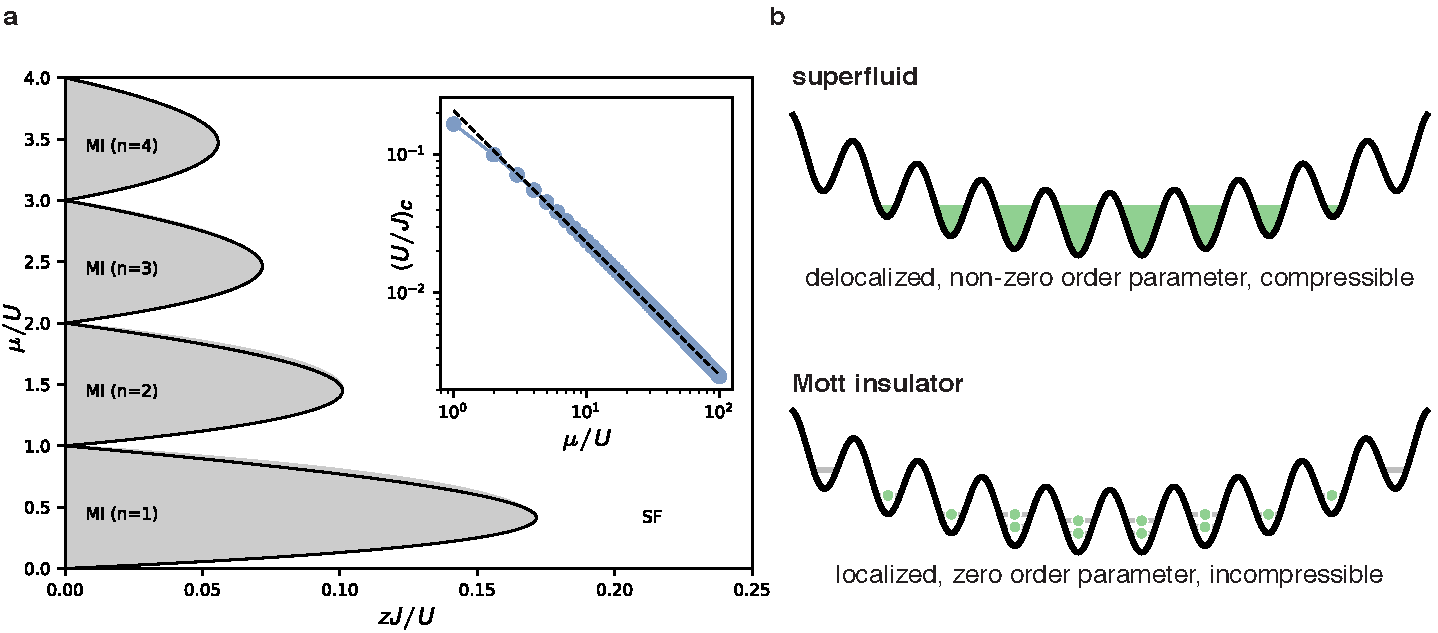
\includegraphics[width=\columnwidth]{figures/ch1/MeanFieldPhaseDiag/MeanFieldDiag_v3.pdf} 
		\caption{\textbf{Mean-field phase diagram. a)} The mean-field phase diagram is shown here for the break down of the superfluid phase into the Mott-insulating lobes (gray) as a function of $J/U$ and $\mu/U$. The coordination number, $z$, corresponds to the number of neighboring sites in a system and in this way accounts for dimensionality. This phase diagram works relatively well for $\geq 2$ spatial dimensions. The inset is a plot of the scaling of the peak of the Mott lobes as a function of $\mu/U$ and demonstrates its suppression with increase in filling $\nu^{-1}$. \textbf{b)} These illustrations demonstrate the qualitative features of the regimes of this phase diagram: i) a superfluid regime which is described by delocalized particles, gapless excitations (for dimensionality $\geq 2$), and non-zero order parameter and ii) a Mott-insulating regime where the particles are localized by inter-particle interactions, the order parameter is zero, and the state contains a finite gap.}
		\label{fig:MF}	
\end{figure}

It can be seen intuitively that the critical, finite value of ${U/J}_c$ depends on the on-site occupation number by comparing the kinetic energy scales to the gap in the system. We first start in a Mott-insulating plateau $|\Psi_{MI} \rangle$ with $n$ atoms per site which has a total energy of $E_0=L\cdot \frac{U}{2} n (n-1)$. The first excitation from this state involves moving an atom from site $i$ to its neighbor and has a total energy of $E_1 = (L-2) \cdot \frac{U}{2} n (n-1) + \frac{U}{2}(n+1)(n) + \frac{U}{2}(n-1)(n-2)$. The gap between these two states is given by $\Delta = E_1 - E_0 = U$ and notably is independent of the on-site occupation number $n_i$. Since the atoms are bosonic and identical, the kinetic energy term $J$ that connects these two states has a bosonic enhancement factor of $\sim n$ and means that the relevant comparison for distinguishing these two phases is $(U/J)_c \propto U/(n J)$. The peaks of the lobes in Fig.~\ref{fig:MF} and are plotted as a function of half integer chemical potential in the inset and agree with a power law exponent $n^{-1}$.

\section{Discussion: beyond tight-binding Bose-Hubbard}

The derivations of the chapter encompass the simplest incarnation of physics relating to a solid state physics system. We derived how a single-particle is diagonalized within a rather simple, but very physically relevant sinusoidal lattice. Incorporating more complex lattice geometries is conceptually the same but can lead to subtle changes in the band structure such as a honeycomb lattice which harbors Dirac points \cite{Geim2007}.

Additionally, even within the currently studied model, when not residing deep in the tight-binding limit, one needs to include the hopping terms to non-nearest neighboring sites to accurately describe the observed physics in the lattice \cite{Preiss2015,Preiss2015QW} (\S \ref{sec:qwcal}). In the case of relatively strong inter-particle interactions, energy shifts from high on-site occupancy can induce hybridization with higher bands and create anharmonic, on-site occupation number dependent changes in the interaction energy \cite{Ma2014}.

The presence of significant on-site, or inter-site potential deviations from disorder in the optical potential can additionally modify the canonical Bose-Hubbard parameters considered earlier. While the predominant deviation comes in directly as on-site energy offsets, $h_i$, the fractional change to the lattice depth between sites will also create a distribution of $J_i$ values, and the fractional change to local site curvature will incur small changes of the interaction strength $U_i$. This is systematically explored for an optical speckle disorder in \emph{White, et al.}\cite{White2009}. Later in this thesis, we will also apply an engineered on-site potential distribution derived from a quasi-periodic potential with respect to the physics lattice. We found that the variation in Bose-Hubbard parameters in this regime were negligible other than the on-site offsets $h_i$ (\S \ref{sec:ch5}).

Lastly, several experimental groups have moved on to atoms from the lanthanide group that host a large number of useful internal states and additionally harbor a strong dipolar magnetic moment that is $\approx 10 \times$ larger than that of standard alkali atoms. These magnetic atoms admit a whole host of interesting quantum phases within optical lattice systems and can be included in the Bose-Hubbard model as additional terms. This construction has been termed the extended Bose-Hubbard model with some recent theoretical interest and experimental progress \cite{Dutta2015,Baier2016}.
 
 
%\section{Beyond flat, tight-binding Bose-Hubbard}
%
%Bose-Glass?
%
%off-site interaction, more than nearest neighbor tunneling, dipole moments?
%
%Disorder effects on J and U cite De Marco, high-order tunneling, tilt and tunneling to higher bands
%
%heating rates, probably refer to appendix




% For an example of a full page figure, see Fig.~\ref{fig:myFullPageFigure}.


%\texttt{This is a line of code.}






